
\documentclass[
	% -- opções da classe memoir --
	12pt,				% tamanho da fonte
	openright,			% capítulos começam em pág ímpar (insere página vazia caso preciso)
	oneside,			% para impressão em verso e anverso.  Usar twoside
	a4paper,			% tamanho do papel. 
	%normalfigtabnum,
	%pnumromarab,
	% -- opções da classe abntex2 --
	chapter=Title,		% títulos de capítulos convertidos em letras maiúsculas
	%section=TITLE,		% títulos de seções convertidos em letras maiúsculas
	%subsection=TITLE,	% títulos de subseções convertidos em letras maiúsculas
	%subsubsection=TITLE,% títulos de subsubseções convertidos em letras maiúsculas
	% -- opções do pacote babel --
	english,			% idioma adicional para hifenização
	french,				% idioma adicional para hifenização
	spanish,			% idioma adicional para hifenização
	brazil,				% o último idioma é o principal do documento
]{abntex2}

\setlrmarginsandblock{3cm}{2cm}{*}
\setulmarginsandblock{3cm}{2cm}{*}
\checkandfixthelayout


% ---------------------------------------------------------------------------------
%                                   PACOTES
% ---------------------------------------------------------------------------------

% ---
% Pacotes básicos 
% ---
\usepackage{acro}
\usepackage{mathptmx}			% Usa a fonte Times New Roman
\usepackage[T1]{fontenc}		% Selecao de codigos de fonte.
\usepackage{lastpage}			% Usado pela Ficha catalográfica
\usepackage{indentfirst}		% Indenta o primeiro parágrafo de cada seção.
\usepackage{xcolor,colortbl}	% Controle das cores
\usepackage{graphicx}			% Inclusão de gráficos
\usepackage{microtype} 			% para melhorias de justificação
\usepackage{hyperref}
\usepackage{subfig}
\usepackage{epigraph}
\usepackage{url}
\usepackage{placeins}
\newcommand*{\rom}[1]{\expandafter\@slowromancap\romannumeral #1@}
\usepackage{multirow}
\usepackage[figuresright]{rotating}
\usepackage{chemfig}
\usepackage{amsmath}
\usepackage{amssymb}
\usepackage{enumitem}
\usepackage{bigints}
\usepackage{listings}
\usepackage{etoolbox}
\usepackage[final]{pdfpages}
\usepackage{bigstrut}
\usepackage{mathtools}
\usepackage{gensymb}
\usepackage{epsfig}
\usepackage{booktabs}
\usepackage{longtable}
\usepackage[bottom]{footmisc}
\usepackage{float}
\DeclareUnicodeCharacter{00A0}{ }
\renewcommand{\sfdefault}{\rmdefault}

% ---
% Pacotes adicionais, usados apenas no âmbito do Modelo Canônico do abnteX2
% ---
\usepackage{lipsum}				% para geração de dummy text
% ---

% ---
% Pacotes de citações
% ---
\usepackage[brazilian,hyperpageref]{backref}	 % Paginas com as citações na bibl
\usepackage[alf,abnt-emphasize=bf,abnt-etal-text=emph,bibjustif]{abntex2cite}  % Citações padrão ABNT


% ---------------------------------------------------------------------------------
%                          CONFIGURAÇÕES DOS PACOTES
% ---------------------------------------------------------------------------------

% ---
% Configurações do pacote backref
%
% Para desativar, tire o comentário de \begin{comment} e \end{comment} 
% das próximas linhas e comente a linha \usepackage[brazilian,hyperpageref]{backref}
% acima.
% ---

%\begin{comment}
% ---
% Configurações do pacote backref
% Usado sem a opção hyperpageref de backref
\renewcommand{\backrefpagesname}{Citado na(s) página(s):~}
% Texto padrão antes do número das páginas
\renewcommand{\backref}{}
% Define os textos da citação
\renewcommand*{\backrefalt}[4]{
	\ifcase #1 %
	Nenhuma citação no texto.%
	\or
	Citado na página #2.%
	\else
	Citado #1 vezes nas páginas #2.%
	\fi}%
% ---
%\end{comment}


% listagens
\definecolor{corComentario}{RGB}{150,150,150}
\definecolor{corString}{RGB}{206,123,0}
\definecolor{corPalavraChave}{RGB}{0,0,230}

\lstset{
	numbers=left,
	stepnumber=1,
	firstnumber=1,
	numberstyle=\footnotesize,
	extendedchars=true,
	breaklines=true,
	lineskip=0pt,
	frame=tb,
	basicstyle=\ttfamily\footnotesize,
	showstringspaces=false,
	stringstyle=\color{corString},
	commentstyle=\color{corComentario},
	keywordstyle=\color{corPalavraChave}
}

\newcolumntype{Y}{>{\centering\arraybackslash}X}

\newcommand{\ano}[1]{\def \oano {#1}}
\newcommand{\imprimirano}{\oano}

\newcommand{\mes}[1]{\def \omes {#1}}
\newcommand{\imprimirmes}{\omes}

\newcommand{\subtitulo}[1]{\def \osubtitulo {#1}}
\newcommand{\imprimirsubtitulo}{\osubtitulo}

\newcommand{\area}[1]{\def \aarea {#1}}
\newcommand{\imprimirarea}{\aarea}

\renewcommand{\coorientador}[1]{\def \ocoorientador {#1}}
\renewcommand{\imprimircoorientador}{\ocoorientador}

\newcommand{\grau}[1]{\def \ograu {#1}}
\newcommand{\imprimirgrau}{\ograu}

\newcommand{\curso}[1]{\def \ocurso {#1}}
\newcommand{\imprimircurso}{\ocurso}


% ---
% Informações de dados para CAPA e FOLHA DE ROSTO
% ---

\curso{Bacharelado em Engenharia De Computação}
\grau{Bacharel em Engenharia De Computação}
% ---------- 
% acronimos
%-----------
\DeclareAcronym{ssh}{
  short = SSH ,
  long  = Secure Shell,
  sort  =  S,
}
\DeclareAcronym{p2p}{
  short = P2P ,
  long  = Peer-to-Peer,
  sort  =  P,
}
\DeclareAcronym{seed}{
  short = Seeds ,
  long  = máquinas que estão compartilhando o arquivo .torrent,
  sort  =  P,
}

\titulo{Transferência de arquivos em redes P2P}

% caso não haja subtítulo, comente a linha abaixo
% \subtitulo{Subtítulo}

\tipotrabalho{}
\area{Área}

\autor{
Carlos Eduardo do Prado Silva – 190715\newline
Eduardo Campos Gonçalves – 190306\newline
Gabriel Maciel Silvério – 190654\newline
João Victor da Costa Wudarski - 190823 (Turma - CP302TIN1)\newline
Johanna Bernecker – 190737\newline
Matheus Bernardo Frate – 190110\newline
Vitor Guilherme Sanches Magnani de Sobral – 190093
}
\orientador{Profº Marcos Fabio Jardini}

% caso não haja coorientador, comente a linha abaixo
% \coorientador{Coorientador}

\local{Sorocaba - Sp}
\mes{outubro}
\ano{2022}

\instituicao{%
	Centro Universitário Facens
	\par
	Engenharia De Computação
}

\preambulo{\imprimirtipotrabalho\ Projeto de pesquisa apresentado ao Curso de Bacharelado em Engenharia da Computação do centro universitário Facens.
}
% ---


% ---
% Configurações de aparência do PDF final
% ---

% alterando o aspecto da cor azul
\definecolor{blue}{RGB}{41,5,195}

% informações do PDF
\makeatletter
\hypersetup{
	%pagebackref=true,
	pdftitle={\@title}, 
	pdfauthor={\@author},
	pdfsubject={\imprimirpreambulo},
	pdfcreator={Nome Completo},
	pdfkeywords={Palavra chave 1}{Palavra chave 2}{Palavra chave 3}{Palavra chave n}, 
	colorlinks=true,       		% false: boxed links; true: colored links
	linkcolor=black,          	% color of internal links
	citecolor=black,       		% color of links to bibliography
	filecolor=black,      		% color of file links
	urlcolor=black,
	bookmarksdepth=4,
}
\makeatother
% --- 11
% ---
% Comandos do autor
% ---

% comando para inserir autor e ano
\newcommand{\citeauthorandyear}[1]{\citeauthoronline{#1} (\citeyear{#1})}


% ---
% Novo list of (listings) para Quadros
% ---



% configurações para atender às regras da ABNT
\setfloatadjustment{quadro}{\centering}
%\counterwithout{quadro}{chapter}
%\renewcommand{\cftquadroname}{\quadroname\space} 
%\renewcommand*{\cftquadroaftersnum}{\hfill--\hfill}

% Configuração de posicionamento padrão:
\setfloatlocations{quadro}{hbtp}



% --- 
% Espaçamentos entre linhas e parágrafos 
% --- 

% O tamanho do parágrafo é dado por:
\setlength{\parindent}{1.3cm}

% Controle do espaçamento entre um parágrafo e outro:
\setlength{\parskip}{0.2cm}  % tente também \onelineskip

% ---
% compila o indice
% ---
\makeindex
% ---







% ---------------------------------------------------------------------------------
%                                   INÍCIO DO DOCUMENTO
% ---------------------------------------------------------------------------------
\begin{document}
\newcommand{\quadroname}{Quadro}
\newcommand{\listofquadrosname}{\normalsize \bfseries LISTA DE QUADROS}
\renewcommand{\listadesimbolosname}{\normalsize \bfseries  LISTA DE SÍMBOLOS}
\renewcommand{\listadesiglasname}{\normalsize \bfseries LISTA DE ABREVIATURAS E SIGLAS}
\renewcommand{\agradecimentosname}{\normalsize \bfseries AGRADECIMENTOS}
\renewcommand{\resumoname}{\normalsize \bfseries RESUMO}
\addto\captionsbrazil{\renewcommand{\listfigurename}{\normalsize \bfseries LISTA DE FIGURAS}}
\addto\captionsbrazil{\renewcommand{\listtablename}{\normalsize \bfseries LISTA DE TABELAS}}
\addto\captionsbrazil{\renewcommand{\bibname}{\normalsize \bfseries REFERÊNCIAS}}
\addto\captionsbrazil{\renewcommand{\contentsname}{\normalsize \bfseries SUMÁRIO}}

% Seleciona o idioma do documento (conforme pacotes do babel)
%
% Retira espaço extra obsoleto entre as frases.

\selectlanguage{brazil}
\frenchspacing 




% ---------------------------------------------------------------------------------
%                                   ELEMENTOS PRÉ-TEXTUAIS
% ---------------------------------------------------------------------------------
%\pretextual

% ---
% Capa
% ---
%\imprimircapa
% capa personalizada

\begin{center}
	
	\center
	
\includegraphics[width=0.2\textwidth]{logo_facens.png}
	\vspace{0.5cm}
	\\
	\ABNTEXchapterfont\textsc{\textbf{\MakeUppercase{\imprimirinstituicao}}}
	\vspace{3.5cm}
	
    \center
    \ABNTEXchapterfont\textsc{\MakeUppercase{\textbf{\imprimirautor}}}
	\vspace{3.5cm}
	
    \ABNTEXchapterfont\textsc{\MakeUppercase{\textbf{\imprimirtitulo\ifdef{\osubtitulo}{:}{}}}}
    
    \ifdef{\osubtitulo}{\MakeUppercase{\ABNTEXchapterfont\imprimirsubtitulo}}{}
	\vfill
	
	\center
        \normalsize
   		Orientador: \imprimirorientador
   		\vfill
	\textsc{\MakeUppercase{\textbf{\imprimirlocal}}}
	
	\textsc{\MakeUppercase{\textbf{\imprimirano}}}
	
	\vspace*{2cm}
	
\end{center}

\cleardoublepage


% ---

% ---
% Folha de rosto
% (o * indica que haverá a ficha bibliográfica)
% ---
%\imprimirfolhaderosto*
% \begin{center}
   	
   	\ABNTEXchapterfont\textsc{\MakeUppercase{\textbf{\imprimirautor}}}
   	\vspace{2.5cm}
   	
    \ABNTEXchapterfont\textsc{\MakeUppercase{\textbf{\imprimirtitulo\ifdef{\osubtitulo}{:}{}}}}
                           
    \ifdef{\osubtitulo}{\MakeUppercase{\ABNTEXchapterfont\imprimirsubtitulo}}{}
   	\vspace{2.5cm}
   	   	
   	\hspace{.42\textwidth}
   	\begin{minipage}{.55\textwidth}
   		\SingleSpacing
   		\small\imprimirpreambulo
   		
   		\vspace{\onelineskip}
   	
   		
   	\end{minipage}%
   		\center
        \normalsize
   		Orientador: \imprimirorientador
   		
        \ifdef{\ocoorientador}{
     		\vspace{\onelineskip}
   		
    		Coorientador: \imprimircoorientador
        }{}
    \vfill
   	
	\textsc{\MakeUppercase{\textbf{\imprimirlocal}}}
	
	\textsc{\MakeUppercase{\textbf{\imprimirano}}}
   	
   	\vspace*{2cm}
   	\pagebreak
\end{center}

% ---
% inserir lista de ilustrações
% ---
\pdfbookmark[0]{\listfigurename}{Lista de Figuras}
\listoffigures*
\cleardoublepage

% ---
% inserir lista de abreviaturas e siglas
% ---
% \input{pre10ListaSiglas}
% ---
\printacronyms[name=Glossário]
\cleardoublepage
% ---
% inserir o sumário
% ---
%\pdfbookmark[0]{\contentsname}{toc}
\tableofcontents*
\cleardoublepage


% ---
% Resumos
% ---
% \setlength{\absparsep}{18pt} % ajusta o espaçamento dos parágrafos do resumo
\begin{resumo}
	
	Resumo
	
	\vspace{\onelineskip}
	
	\textbf{Palavras-chave}: 1. Palavra-chave  2. Palavra-chave 3. Palavra-chave.
	
\end{resumo}

% ---------------------------------------------------------------------------------
%                                  ELEMENTOS TEXTUAIS
% ---------------------------------------------------------------------------------
\textual
\renewcommand{\ABNTEXchapterfont}{\rmfamily\bfseries\MakeUppercase}
\renewcommand{\ABNTEXchapterfontsize}{\normalsize}
\renewcommand{\ABNTEXsectionfont}{\ABNTEXchapterfont}
\renewcommand{\ABNTEXsectionfontsize}{\normalsize}
\renewcommand{\ABNTEXsubsectionfont}{\ABNTEXsectionfont}
\renewcommand{\ABNTEXsubsectionfontsize}{\normalsize}
\renewcommand{\ABNTEXsubsubsectionfont}{\ABNTEXsubsectionfont}
\renewcommand{\ABNTEXsubsubsectionfontsize}{\normalsize}
\renewcommand{\tocheadstart}{\ABNTEXchapterfont}







\chapter{INTRODUÇÃO}
\label{cap:01}
\section{\ac{p2p}}
 
Redes \textit{\ac{p2p}}  são redes virtuais que funcionam na Internet nas quais os membros são equivalentes em funcionalidades, permitindo que os participantes ou pares, compartilhem recursos diretamente, sem envolver um servidor central ou outro tipo de intermediários, dessa forma funcionando com uma arquitetura descentralizada. Como não há um servidor armazenando informações de identificação dos pares, torna-se muito difícil rastrear e identificar um usuário do sistema, garantindo a segurança da rede. O controle de conexões e fluxo de informações em uma rede \ac{p2p} em uma arquitetura distribuída, ou seja, as informações de controle (indexação e descoberta de pares) circulam entre os pares, assim como os dados. \cite{p2p, rocha2004peer}

Existem dois tipos principais de arquitetura, a arquitetura descentralizada, onde cada par dentro da arquitetura são equivalentes em funcionalidades e não existe nenhum nó que controle o fluxo de informações e dados dentro da rede. A segunda principal arquitetura é a Semicentralizada, onde os nós também são equivalentes em funcionalidades mas ao menos um dos nós servirá  ao papel de controle desempenhando uma autoridade dentro da rede.\cite{inproceedings}


\section{Sistemas Distribuidos}
Parte da definição de sistemas distruibuídos é que maquinas diferentes conectadas por uma rede, se comunicam e coordenam suas ações através de mensagens enviadas entre si, e  apresentando-se como um sistema único aos usuários, para isso é ocultado algumas das características e assim sendo definidos como transparentes. As principais formas de transparencias são acessos, localização, migração, relocação, replicação, concorrência e falha. \cite{van2002distributed, coulourisdistributed}


As redes \ac{p2p} conseguem se manter transparentes em concorrência, pois um serviço ou cliente faz requisições em mais de um servidor, já que não possui um servidor centralizado. Dessa mesma forma, é ocultado o lugar onde um recurso está localizado, mantendo também a transparência na replicação, pois permite que várias instâncias dos recursos sejam usadas para aumentar a confiabilidade e desempenho. \cite{van2002distributed}
    
“São sistemas distribuídos compostos de nós interconectados, aptos a se auto-organizar em topologias de rede, com o intuito de compartilhar recursos, como conteúdo, ciclos de CPU, largura de banda e armazenamento, com a capacidade de adaptação a faltas e acomodação a um número variável de nós, ao mesmo tempo que mantém a conectividade e o desempenho em níveis aceitáveis, sem a necessidade de suporte ou intermediação de um servidor centralizado.” \cite{androutsellis2004survey}

\chapter{Objetivos}
\label{cap:02}
Dessa forma, este trabalho se propõe a realizar um exemplo de rede \ac{p2p} que mantém a transparência de concorrência e replicação durante uma transmissão de arquivos, onde será feita uma solicitação de um arquivo atráves do software QBittorrent, que está presente em mais de uma máquina, sendo o envio do arquivo feito por todas as instâncias, aumentando a confiabilidade e desempenho no envio.
 
\chapter{RESULTADOS E DISCUSSÃO}
\label{cap:04}
Para o desenvolvimento foi utilizado duas maquinas virtuais com o sistema Operacional \textit {OpenSuse}, com o software de transmissão de arquivos atráves do protocolo torrent, qBittorrent, instalado.
Para realizar um acesso remoto à essas máquinas, foi utilizado o cliente de conexão  \textit{\ac{ssh}} Putty e nele configurado a opção de controle SSH X11 \textit {forwarding}, para que a a interface gráfica da máquina virtual fosse aberta pela maquina host.

Foi utilizado o mesmo arquivo .torrent em ambas as máquinas e os testes não foram feito de forma simultaneas para que não houvesse distribuição de banda e elas pudessem ter o máximo desempenho nos testes, dessa forma é possível analisar as transparências de concorrência e replicação. 

Na primeira máquina virtual foi realizado o download do arquivo conectando com todos as \ac{seed} disponíveis. Quando conectado a 10 \ac{seed}, foi obtido uma disponibilidade do arquivo de 10.046, e uma velocidade média de download de 8.2MiB/S, conforme a figura \ref{fig:disponibilidade 10 seeds}  
\begin{figure}[!htb]
\centering
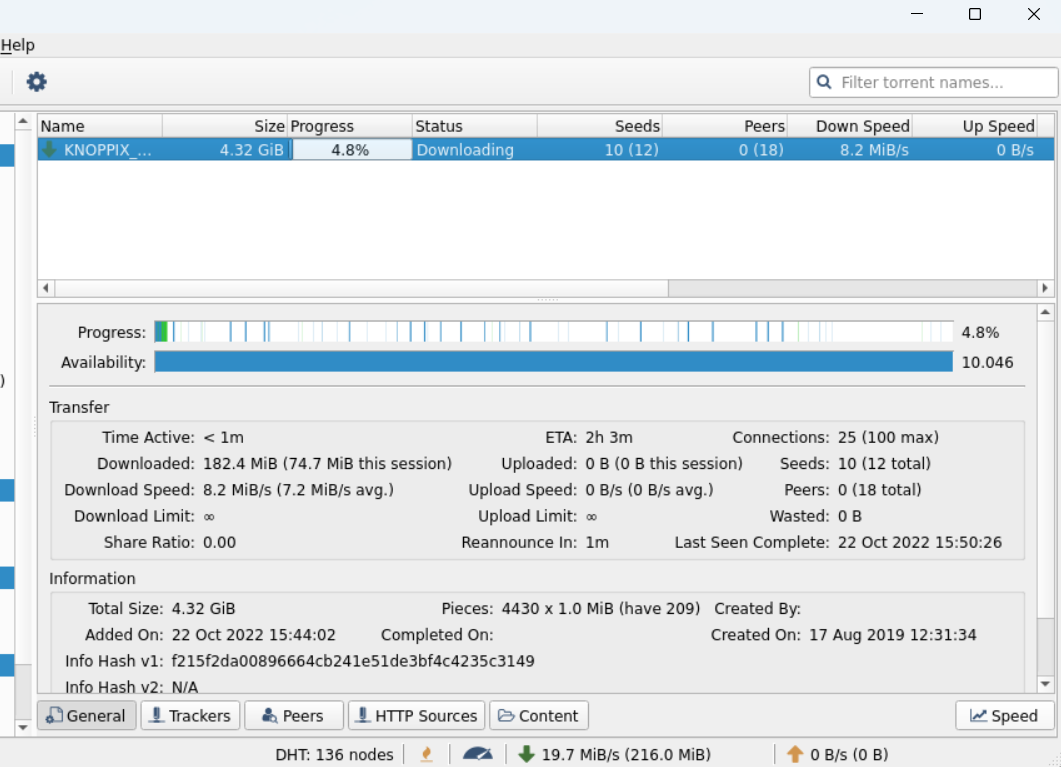
\includegraphics[width=0.6\textwidth]{./images/disponibilidade 10 seeds.png}
\caption{Disponibilidade do arquivo com 10 seeds}
\label{fig:disponibilidade 10 seeds}
\end{figure}

Na segunda máquina virtual foi limitado a quantidade de peers conectados com o intuito de diminuir a concorrência e o desempenho, Quando conectado a 5 \ac{seed}, foi obtido uma disponibilidade de 5.256, e uma velocidade média de donwload de 1.6MiB/S, conforme a figura \ref{fig:disponibilidade_5_seeds}
\begin{figure}[!htb]
\centering
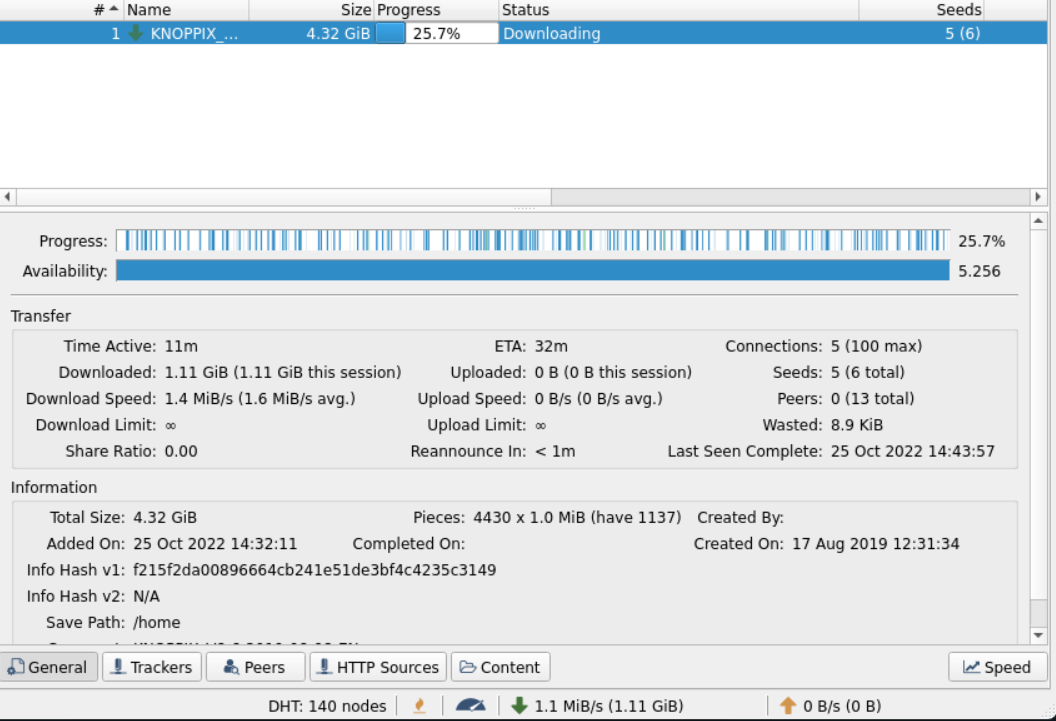
\includegraphics[width=0.65\textwidth]{./images/disponibilidade 5 seeds.png} 
\caption{Disponibilidade do arquivo com 5 seeds}
\label{fig:disponibilidade_5_seeds}
\end{figure}

Foi realizado um teste sobre a disponibilidade e velocidade de transmissão do arquivo .torrent, quando conectado a somente um seed, mostrando um gráfico de velocidade de download estabilizado com velocidade de 832.1KiB/S após a mudança para somente 1 seed conforme a figura \ref{fig:velocidade_1_seed}.
\begin{figure}[!htb]
\centering
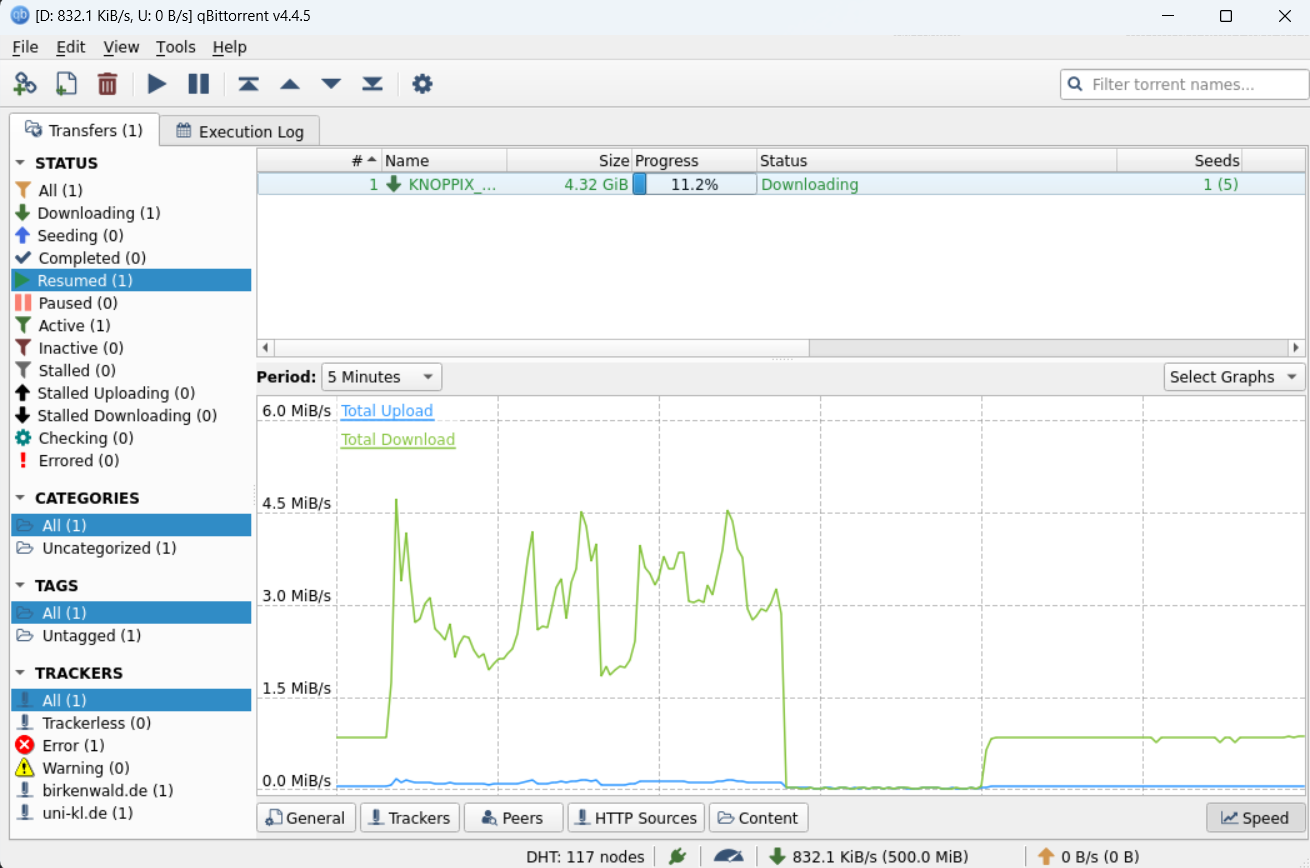
\includegraphics[width=0.7\textwidth]{./images/velocidade download 1 seed.png}
\caption{Velocidade de Download com 1 seed}
\label{fig:velocidade_1_seed}
\end{figure}
\chapter{CONCLUSÕES}
\label{cap:05}
dessa forma é possível analisar as transparências de concorrência e replicação. 
Conforme as informações nas figuras \ref{fig:disponibilidade 10 seeds} e \ref{fig:disponibilidade_5_seeds}, é possível ver a transparência de replicação, onde o mesmo objeto está replicado em varias máquinas diferentes, que são os \ac{seed}, mas a transferência é feita de maneira única. 

No desempenho da velocidade de download do arquivo foi possível notar diferenças com o aumento da quantidade de \ac{seed} conectados, com 5 \ac{seed} a velocidade média obtida foi de 2 MiB/S, representado pela figura \ref{fig:geral_5_seeds}, enquanto com 12 \ac{seed}, foi obtido uma velocidade média de 25 MiB/S, representado pela figura \ref{fig:geral_12_seeds}.

A quantidade de \ac{seed} conectados transmitindo arquivos simultaneamente, mostram que as redes \ac{p2p} são transparentes em concorrência, pois os arquivos compartilhados são transmitidos de diversas máquinas diferentes enquanto no cliente é realizado o download de forma única sem ficar evidente que cada parte do arquivo está sendo transmitido por uma máquina diferente. 

Conclui-se que as redes \ac{p2p} se mantém transparentes em concorrência e replicação, se encaixando em sistemas distribuídos. 
\begin{figure}[!htb]
\centering
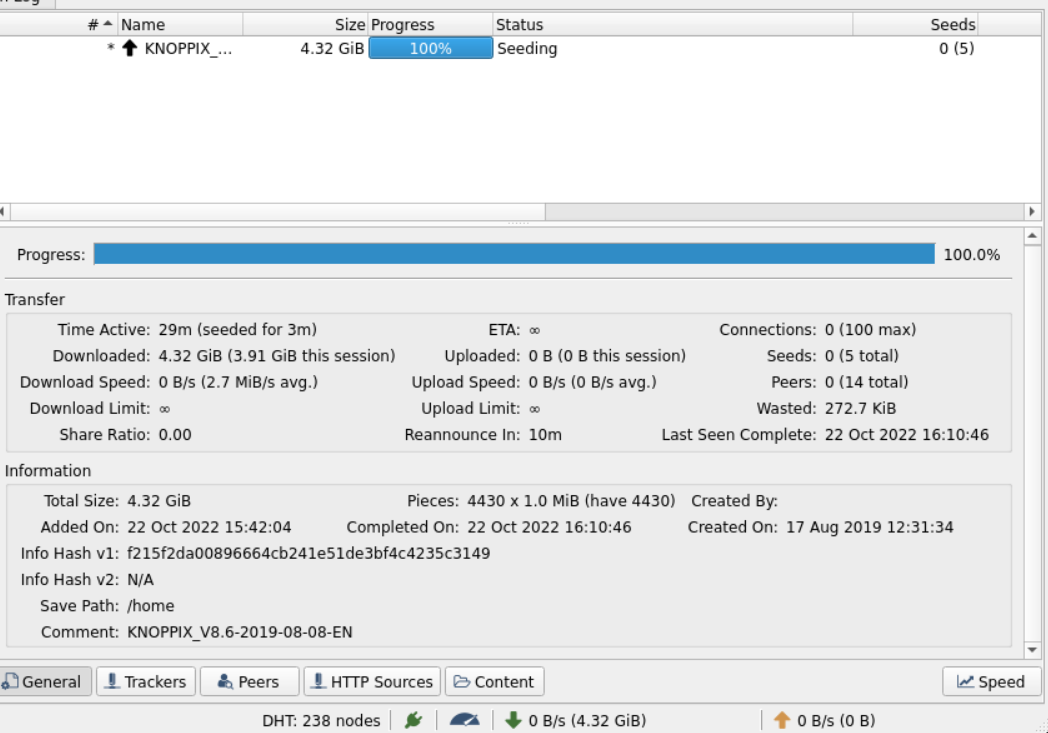
\includegraphics[width=0.7\textwidth]{./images/5 seeds geral.png}
\caption{Informações Gerais de download com 5 seeds}
\label{fig:geral_5_seeds}
\end{figure}

\begin{figure}[!htb]
\centering
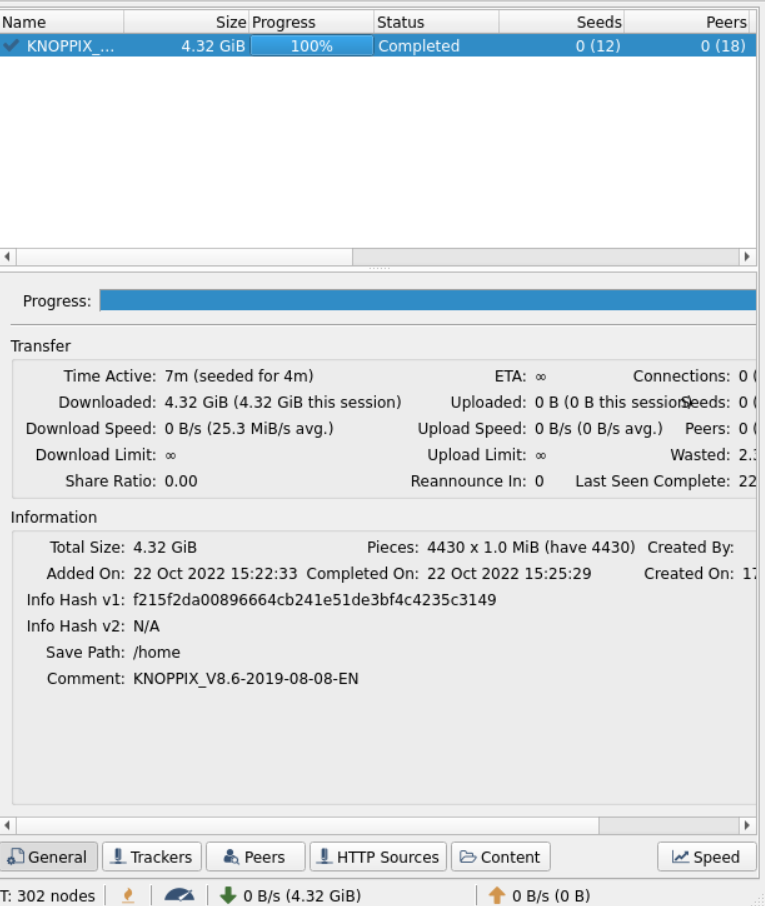
\includegraphics[width=0.7\textwidth]{./images/geral 12 seeds.png}
\caption{Informações Gerais de download com 12 seeds}
\label{fig:geral_12_seeds}
\end{figure}
%\input{capitulo06Cronograma}





% ---------------------------------------------------------------------------------
%                                 ELEMENTOS PÓS-TEXTUAIS
% ---------------------------------------------------------------------------------
% \postextual

% ----------------------------------------------------------
% Referências bibliográficas
% ----------------------------------------------------------
\bibliography{Referencias}

\end{document}
